
\documentclass[border=10pt, 12pt]{standalone}
\usepackage[svgnames]{xcolor}
\usepackage{amsmath}
\usepackage{pgfplots}
\pgfplotsset{compat=newest}
\usepackage[sfdefault]{FiraSans}
\usepackage{FiraMono}
\renewcommand*\familydefault{\sfdefault}
\begin{document}
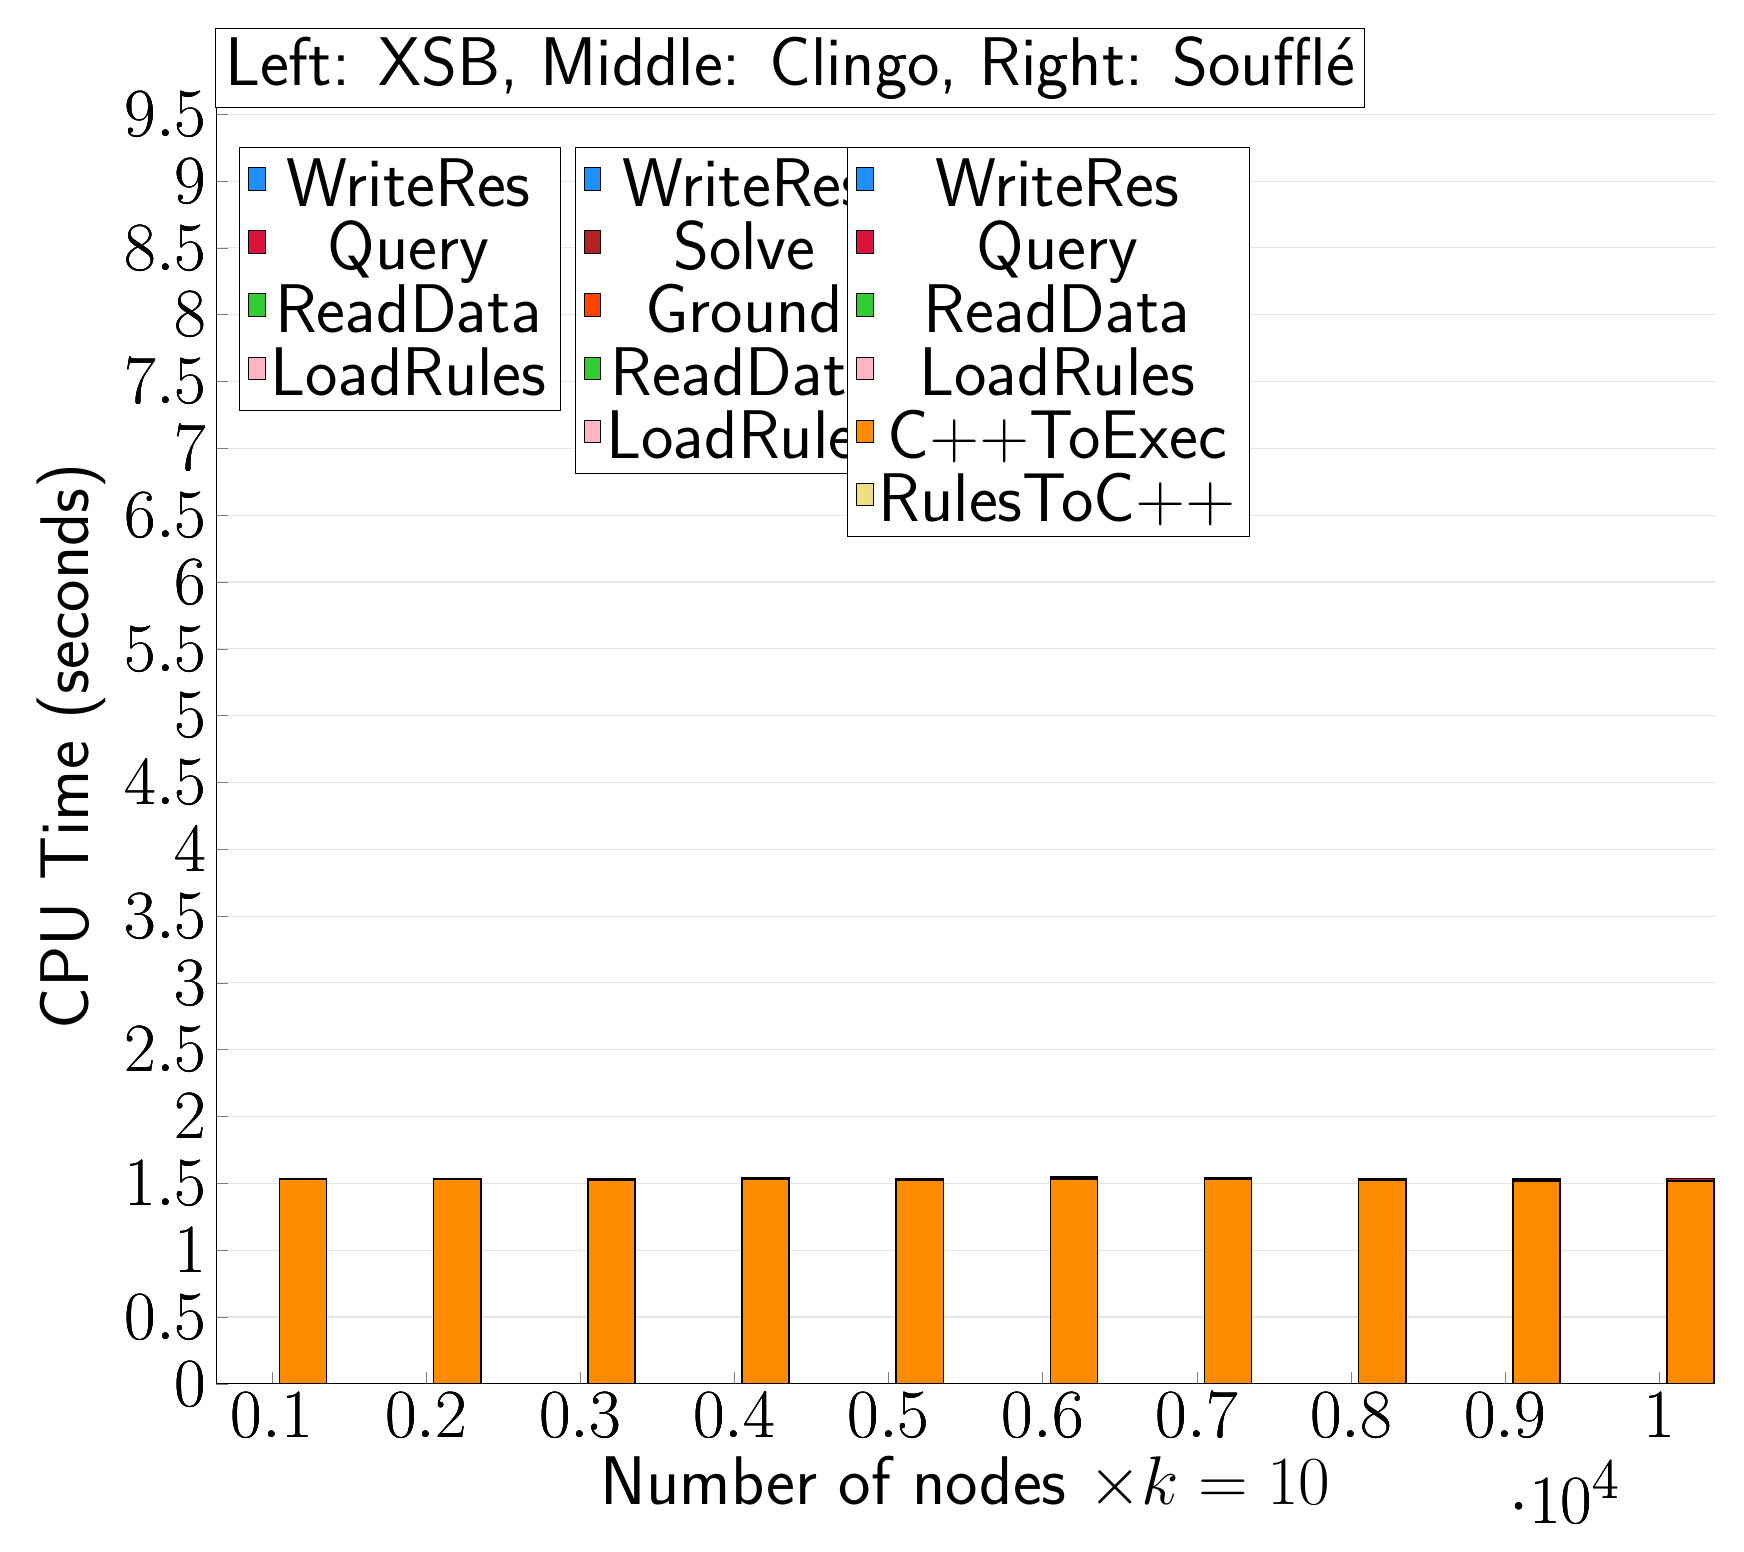
\begin{tikzpicture}
                        \begin{axis}[bar shift=-24.3pt, 
   ybar stacked,
   width=1.7\textwidth,
   bar width=0.6cm,
   ymajorgrids, tick align=inside,
   major grid style={draw=gray!20},
   xtick=data,
   ymin=0, ymax=9.544,
   axis x line*=bottom,
   axis y line*=left,
   enlarge x limits=0.04,
   legend style={
       at={(0.23, 0.97)},
       anchor=north east,
       legend columns=1,
       font=\Huge,
   },
   ylabel={CPU Time (seconds)},
   xlabel={Number of nodes $\times k=10$},
   label style={font=\Huge},
   tick label style={font=\Huge},
]
\addlegendimage{fill=DodgerBlue, draw=black, line width=0.2pt}
\addlegendentry{WriteRes}
\addlegendimage{fill=Crimson, draw=black, line width=0.2pt}
\addlegendentry{Query}
\addlegendimage{fill=LimeGreen, draw=black, line width=0.2pt}
\addlegendentry{ReadData}
\addlegendimage{fill=LightPink, draw=black, line width=0.2pt}
\addlegendentry{LoadRules}
\addplot +[fill=LightPink, draw=black, line width=0.55pt] coordinates {
(1000, 0.0005676)
(2000, 0.0005565999999999993)
(3000, 0.0005558000000000005)
(4000, 0.0005529999999999996)
(5000, 0.0005516000000000004)
(6000, 0.0005591999999999998)
(7000, 0.0005585999999999997)
(8000, 0.0005554)
(9000, 0.0005586000000000005)
(10000, 0.0005552000000000003)
};
\addplot +[fill=LimeGreen, draw=black, line width=0.55pt] coordinates {
(1000, 0.00020420000000000022)
(2000, 0.00028440000000000057)
(3000, 0.00036939999999999987)
(4000, 0.0004438)
(5000, 0.0005296000000000001)
(6000, 0.0005970000000000002)
(7000, 0.0006780000000000004)
(8000, 0.0007575999999999998)
(9000, 0.0008330000000000001)
(10000, 0.0009283999999999997)
};
\addplot +[fill=Crimson, draw=black, line width=0.55pt] coordinates {
(1000, 8.599999999999935e-06)
(2000, 7.999999999999676e-06)
(3000, 9.000000000000329e-06)
(4000, 9.39999999999969e-06)
(5000, 8.599999999999926e-06)
(6000, 8.600000000000273e-06)
(7000, 7.999999999999676e-06)
(8000, 8.400000000000074e-06)
(9000, 8.79999999999978e-06)
(10000, 8.399999999999728e-06)
};
\addplot +[fill=DodgerBlue, draw=black, line width=0.55pt] coordinates {
(1000, 6.240000000000065e-05)
(2000, 6.520000000000032e-05)
(3000, 6.540000000000017e-05)
(4000, 6.320000000000007e-05)
(5000, 6.399999999999946e-05)
(6000, 6.440000000000018e-05)
(7000, 6.300000000000054e-05)
(8000, 6.359999999999974e-05)
(9000, 6.40000000000005e-05)
(10000, 6.560000000000001e-05)
};
\end{axis}

\begin{axis}[bar shift=-6.5pt, 
   ybar stacked,
   width=1.7\textwidth,
   bar width=0.6cm,
   ymajorgrids, tick align=inside,
   major grid style={draw=none},
   xtick=data,
   ymin=0, ymax=9.544,
   axis x line*=none,
   axis y line*=none,
   enlarge x limits=0.04,
   legend style={
       at={(0.454, 0.97)},
       anchor=north east,
       legend columns=1,
       font=\Huge,
   },
   label style={font=\Huge},
   tick label style={font=\Huge},
]
\addlegendimage{fill=DodgerBlue, draw=black, line width=0.2pt}
\addlegendentry{WriteRes}
\addlegendimage{fill=FireBrick, draw=black, line width=0.2pt}
\addlegendentry{Solve}
\addlegendimage{fill=OrangeRed, draw=black, line width=0.2pt}
\addlegendentry{Ground}
\addlegendimage{fill=LimeGreen, draw=black, line width=0.2pt}
\addlegendentry{ReadData}
\addlegendimage{fill=LightPink, draw=black, line width=0.2pt}
\addlegendentry{LoadRules}
\addplot +[fill=LightPink, draw=black, line width=0.55pt] coordinates {
(1000, 0.0)
(2000, 0.0)
(3000, 0.0)
(4000, 0.0)
(5000, 0.0)
(6000, 0.0)
(7000, 0.0)
(8000, 0.0)
(9000, 0.0)
(10000, 0.0)
};
\addplot +[fill=LimeGreen, draw=black, line width=0.55pt] coordinates {
(1000, 0.0)
(2000, 0.0)
(3000, 0.0)
(4000, 0.0)
(5000, 0.0)
(6000, 0.0)
(7000, 0.0)
(8000, 0.0)
(9000, 0.0)
(10000, 0.0)
};
\addplot +[fill=OrangeRed, draw=black, line width=0.55pt] coordinates {
(1000, 0.0)
(2000, 0.0)
(3000, 0.0)
(4000, 0.0020000000000000018)
(5000, 0.0)
(6000, 0.0)
(7000, 0.0)
(8000, 0.0)
(9000, 0.0040000000000000036)
(10000, 0.0)
};
\addplot +[fill=FireBrick, draw=black, line width=0.55pt] coordinates {
(1000, 0.0)
(2000, 0.0)
(3000, 0.0)
(4000, 0.0)
(5000, 0.0)
(6000, 0.0)
(7000, 0.0)
(8000, 0.0)
(9000, 0.0)
(10000, 0.0)
};
\addplot +[fill=DodgerBlue, draw=black, line width=0.55pt] coordinates {
(1000, 0.0)
(2000, 0.0)
(3000, 0.0)
(4000, 0.0)
(5000, 0.0)
(6000, 0.0)
(7000, 0.0)
(8000, 0.0020000000000000018)
(9000, 0.0)
(10000, 0.0)
};
\end{axis}

\begin{axis}[bar shift=11.3pt, 
   ybar stacked,
   width=1.7\textwidth,
   bar width=0.6cm,
   ymajorgrids, tick align=inside,
   major grid style={draw=none},
   xtick=data,
   ymin=0, ymax=9.544,
   axis x line*=none,
   axis y line*=none,
   enlarge x limits=0.04,
   legend style={
       at={(0.69, 0.97)},
       anchor=north east,
       legend columns=1,
       font=\Huge,
   },
   label style={font=\Huge},
   tick label style={font=\Huge},
]
\addlegendimage{fill=DodgerBlue, draw=black, line width=0.2pt}
\addlegendentry{WriteRes}
\addlegendimage{fill=Crimson, draw=black, line width=0.2pt}
\addlegendentry{Query}
\addlegendimage{fill=LimeGreen, draw=black, line width=0.2pt}
\addlegendentry{ReadData}
\addlegendimage{fill=LightPink, draw=black, line width=0.2pt}
\addlegendentry{LoadRules}
\addlegendimage{fill=DarkOrange, draw=black, line width=0.2pt}
\addlegendentry{C++ToExec}
\addlegendimage{fill=LightGoldenrod, draw=black, line width=0.2pt}
\addlegendentry{RulesToC++}
\addplot +[fill=LightGoldenrod, draw=black, line width=0.55pt] coordinates {
(1000, 0.0)
(2000, 0.0020000000000000005)
(3000, 0.0)
(4000, 0.0020000000000000005)
(5000, 0.0)
(6000, 0.0)
(7000, 0.0)
(8000, 0.0)
(9000, 0.0)
(10000, 0.0)
};
\addplot +[fill=DarkOrange, draw=black, line width=0.55pt] coordinates {
(1000, 1.53)
(2000, 1.528)
(3000, 1.5259999999999998)
(4000, 1.53)
(5000, 1.5239999999999998)
(6000, 1.5340000000000003)
(7000, 1.528)
(8000, 1.52)
(9000, 1.5159999999999998)
(10000, 1.516)
};
\addplot +[fill=LightPink, draw=black, line width=0.55pt] coordinates {
(1000, 0.00014680000000000002)
(2000, 0.0001464)
(3000, 0.0001542)
(4000, 0.0001492)
(5000, 0.000142)
(6000, 0.00014)
(7000, 0.0001404)
(8000, 0.00015500000000000003)
(9000, 0.00014160000000000003)
(10000, 0.0001418)
};
\addplot +[fill=LimeGreen, draw=black, line width=0.55pt] coordinates {
(1000, 0.000898)
(2000, 0.0012879999999999999)
(3000, 0.0016018)
(4000, 0.0020879999999999996)
(5000, 0.0024073999999999996)
(6000, 0.0027812)
(7000, 0.0031788)
(8000, 0.003157)
(9000, 0.0037311999999999996)
(10000, 0.0041614)
};
\addplot +[fill=Crimson, draw=black, line width=0.55pt] coordinates {
(1000, 0.0022595999999999996)
(2000, 0.004132800000000001)
(3000, 0.005455999999999999)
(4000, 0.007288)
(5000, 0.0087358)
(6000, 0.010165400000000002)
(7000, 0.011892)
(8000, 0.0121086)
(9000, 0.013916600000000001)
(10000, 0.015652199999999998)
};
\addplot +[fill=DodgerBlue, draw=black, line width=0.55pt] coordinates {
(1000, 0.0004698)
(2000, 0.00045840000000000003)
(3000, 0.0003442)
(4000, 0.0003336)
(5000, 0.0002848)
(6000, 0.0003288)
(7000, 0.00028419999999999997)
(8000, 0.0002558)
(9000, 0.0002808)
(10000, 0.00029660000000000005)
};
\end{axis}


\node[anchor=south, draw, fill=white] at (rel axis cs:0.42,1) {\Huge Left: XSB, Middle: Clingo, Right: Soufflé};
\end{tikzpicture}
\end{document}
                    